\section{Different-content endpoint relations}\label{sec:endpoints}
Up to now the content of a history, the multiset of its labels, was fixed. Here two histories with \emph{different} contents are compared. They can meet at one endpoint only through an arithmetic relation among the multipliers $R(N)$, and this relation is a lattice kernel.

\subsection{The valuation matrix and its kernel}
Fix a finite alphabet $A$ of labels. Let $\mathcal P$ be the set of primes dividing some $N$ or $N+1$ with $N\in A$, and let $V_A=(\Delta_p(N))_{p\in\mathcal P,\,N\in A}$ be the integer matrix of displacement vectors. For a history $h$ over $A$ let $c(h)\in\N^A$ be its content vector.
\begin{theorem}[endpoint equality is a kernel condition]\label{thm:kernel}
Two histories over $A$ from the same source have the same endpoint if and only if $V_A(c-c')=0$.
\end{theorem}
\begin{proof}
The endpoint is $m\prod_N R(N)^{c_N}$. A positive rational is determined by its $p$-adic valuations, $v_p(R(N))=\Delta_p(N)$, and a prime outside $\mathcal P$ has valuation $0$ for every $R(N)$, $N\in A$. Hence the endpoints agree iff $\sum_N(c_N-c'_N)\Delta_p(N)=0$ for all $p\in\mathcal P$.
\end{proof}
\prov{CW-0369}{D4-T1}{PROVED}{FULL}
\emph{Finite check.} Over all words of length $\le6$ from four sources, and on a box of $8\,110\,682$ content pairs of the programme's records, there is no violation (cited; the statement is a theorem, the check only guards the implementation). The content vectors of equal-endpoint histories form a coset of $\ker_{\Z}V_A$ intersected with $\N^A$ (a \emph{toric fibre}).

\begin{theorem}[every kernel vector is realised]\label{thm:realise}
Let $0\ne z\in\ker_{\Z}V_A$, $z=z^+-z^-$ with $z^\pm\ge0$, and let $m=\prod_N N^{|z_N|}$. Then every arrangement of the content $z^+$ and every arrangement of the content $z^-$ is admissible from $m$, and all of these histories have one endpoint, namely $m\prod_N R(N)^{z^+_N}=m\prod_N R(N)^{z^-_N}$. For arrangements $u$ of $z^+$ and $v$ of $z^-$ the pair is simultaneously admissible from a source $m'$ iff $\lcm(K(u),K(v))\mid m'$; the minimal sources of the relation form the antichain of the minimal $\lcm(K(u),K(v))$.
\end{theorem}
\begin{proof}
The content $z^+$ has $P(z^+)=\prod N^{z^+_N}$ dividing $m$, and likewise $P(z^-)$; by \cref{prop:sat} all arrangements are admissible. The endpoints coincide by \cref{thm:kernel}. The simultaneous admissibility criterion is \cref{thm:threshold} applied to $u$ and $v$.
\end{proof}
\prov{CW-0370}{D4-T2}{PROVED}{FULL}
The realising source is sufficient, not minimal. For the kernel vector $z$ below the pair $(2,2,3,3,3,3)$ against $(1^7)$ needs only the source $4$, whereas $\prod N^{|z_N|}=1\cdot2^2\cdot3^4=324$.

\begin{theorem}[the labels $\{1,2,3\}$]\label{thm:123}
$\ker_{\Z}V_{\{1,2,3\}}=\Z\,(7,-2,-4)$; equivalently $R(1)^7=R(2)^2R(3)^4=4^7=16384$.
\end{theorem}
\begin{proof}
Only the primes $2,3$ occur: $R(1)=4$, $R(2)=9/2$, $R(3)=16/3$ give
\[V=\begin{pmatrix}2&-1&4\\0&2&-1\end{pmatrix}\quad(\text{rows }p=2,3;\ \text{columns }N=1,2,3).\]
The rows are independent, so the kernel has rank $1$. From the second row $c_3=2c_2$ and from the first $2c_1-c_2+8c_2=0$, i.e.\ $c_1=-\tfrac72c_2$; the primitive generator is $(7,-2,-4)$. Direct evaluation: $(9/2)^2(16/3)^4=\frac{81}{4}\cdot\frac{65536}{81}=16384=4^7$.
\end{proof}
\prov{CW-0372}{D4-T4}{PROVED}{FULL}
\begin{example}[the benchmark merger from $4$]\label{ex:merger}
From the source $4$ the history $1^7$ passes through $4,16,64,256,1024,4096,16384,65536$. The content $\{2,2,3,3,3,3\}$ has exactly three admissible arrangements from $4$, namely $(2,2,3,3,3,3)$ through $4,18,81,432,2304,12288,65536$, and the arrangements $(2,3,2,3,3,3)$, $(2,3,3,2,3,3)$ (states shown in \cref{fig:merger}). All end at $4^8=65536$. Here $K(1^7)=1$, $K(2,2,3,3,3,3)=4$ and the smallest threshold of the three arrangements is $2$. \stat{finite-exact} in the arrangement count.
\end{example}
\begin{figure}[tbp]\centering
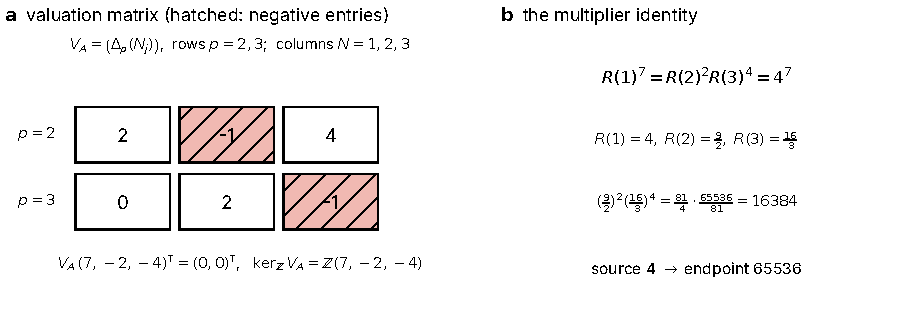
\includegraphics[width=\linewidth]{fig16_valuation_kernel}
\caption{\textbf{The valuation matrix of $\{1,2,3\}$ and the multiplier identity (exact).} (a) The matrix $V_A=(\Delta_p(N))$ with rows $p=2,3$ and columns $N=1,2,3$; entries are exact integers, negative entries are shaded and hatched. $V_A(7,-2,-4)^{\mathsf T}=0$ and the kernel over $\Z$ is $\Z(7,-2,-4)$. (b) The identity $R(1)^7=R(2)^2R(3)^4=4^7$ behind it; source $4$, endpoint $65536$. Theorem illustrated: \cref{thm:123}.}\label{fig:kernel}
\end{figure}
\noindent The figure above is \cref{fig:kernel}; its caption states the exactness of what is drawn.
\begin{figure}[tbp]\centering
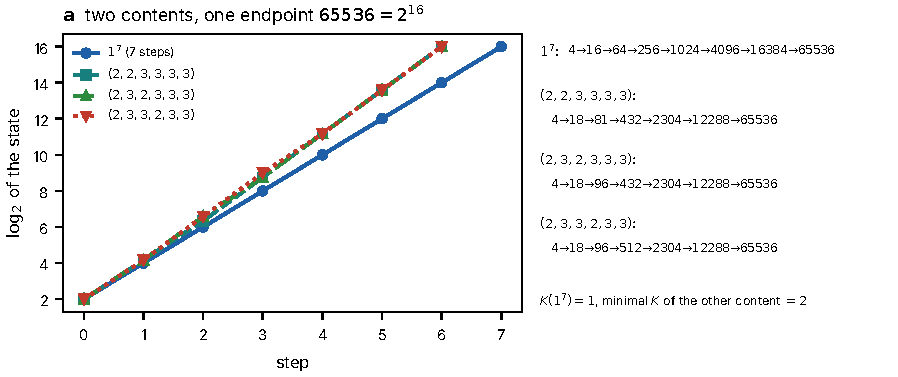
\includegraphics[width=\linewidth]{fig17_two_contents_65536}
\caption{\textbf{Two contents with one endpoint (exact, source $4$, endpoint $65536=2^{16}$).} (a) $\log_2$ of the state against the step for the history $1^7$ (circles, $7$ steps) and the three admissible arrangements of $\{2^2,3^4\}$ (squares, triangles; $6$ steps; dashed, dash-dotted and dotted lines respectively). The curves are different but meet at the endpoint. (b) The exact state sequences. $K(1^7)=1$; the smallest threshold among the three arrangements is $2$. Theorem illustrated: \cref{thm:realise}, \cref{thm:123}.}\label{fig:merger}
\end{figure}

\subsection{Geometry of the recombination: traces, area and closure}
Write $d_N=\Delta(N)\in\Z^{\mathcal P}$ and let the \emph{trace} of a history be the set of its visited states.
\begin{theorem}[trace and area]\label{thm:trace}
\begin{enumerate}[label=(\alph*)]
\item \emph{Trace injectivity.} Distinct histories from one source have distinct traces: the states strictly increase ($R(N)>1$), so ordering the trace recovers the state sequence, and consecutive ratios recover the labels because $R$ is injective.
\item \emph{Area potential.} For a word $w=(N_1,\dots,N_l)$ put $\Omega(w)=\sum_{i<j}d_{N_i}\wedge d_{N_j}$ (a bivector). An adjacent exchange of $N_k=a$ and $N_{k+1}=b$ changes $\Omega$ by exactly $-2\,d_a\wedge d_b$ (sharpening the factor $1$ recorded in the source); a block replacement $u\to v$ with $\sum d_u=\sum d_v$ changes $\Omega$ by $\Omega(v)-\Omega(u)$, independently of the prefix and the suffix. For arrangements of $\{2^2,3^4\}$ with $\mathrm{inv}$ the number of pairs with a $3$ before a $2$,
\[\Omega=\det(d_2,d_3)\,(8-2\,\mathrm{inv})\ (\text{in the }(v_2,v_3)\text{-plane}),\quad\det(d_2,d_3)=-7.\]
\item \emph{Closure triangle.} From the source $4$ the two histories $1^7$ and $(2,2,3^4)$, in the $(v_2,v_3)$-plane, bound the triangle with vertices $(2,0),(0,4),(16,0)$ (sides $2d_2$, $4d_3$ and $7d_1$) of area $28=4\,|\det(d_2,d_3)|$; the two paths meet only at their endpoints.
\end{enumerate}
\end{theorem}
\begin{proof}
(a) was argued above. (b) For an exchange, the terms $d_{N_i}\wedge d_{N_k}+d_{N_i}\wedge d_{N_{k+1}}$ with $i<k$ and $d_{N_k}\wedge d_{N_j}+d_{N_{k+1}}\wedge d_{N_j}$ with $j>k+1$ are symmetric in the exchanged pair, and the single pair term $d_a\wedge d_b$ becomes $d_b\wedge d_a=-d_a\wedge d_b$, which changes $\Omega$ by $-2d_a\wedge d_b$. For a block replacement, the cross terms between a prefix or suffix and the block are of the form $d_{N}\wedge\sum d_u$, and $\sum d_u=\sum d_v$. For $2^2 3^4$: pairs of equal labels contribute $0$; a pair $2$ before $3$ contributes $d_2\wedge d_3=-7$ and a pair $3$ before $2$ contributes $+7$, so $\Omega=-7(8-\mathrm{inv})+7\,\mathrm{inv}$. (c) The trace of $1^7$ is $(2,0),(4,0),\dots,(16,0)$; that of $(2,2,3,3,3,3)$ is $(2,0),(1,2),(0,4),(4,3),(8,2),(12,1),(16,0)$ (exact, verified from the state values). The triangle's area is $\frac12\cdot14\cdot4=28$; the second path stays in $v_3>0$ except at its endpoints.
\end{proof}
\prov{CW-0387}{B-T5}{PROVED}{FULL}
\begin{remark}[what $\Omega$ is and is not]
$\Omega$ is a function on vertices of the swap-and-rewrite graph, so the signed area of every closed combinatorial loop in that graph is $0$ by construction; it measures the \emph{area between two histories}, a weighted inversion statistic, not a homology class. It realises the $1$-skeleton and the bigons of the extended complex; higher cells are not realised as solids, and no coherence cells are present.
\end{remark}
\begin{proposition}[swap diamonds are nondegenerate; finite-exact]\label{prop:nondeg}
No two distinct labels $N<M\le400$ have parallel displacement vectors $d_N\parallel d_M$, so every swap diamond has nonzero area in some coordinate plane. The statement for all $N$ is open. \stat{finite-exact} (recomputed here: $0$ parallel pairs among labels $1,\dots,400$).
\end{proposition}
\prov{CW-0388}{B-T6}{FINITE-EXACT}{FINITE}

\subsection{The cube family}
Let $\mathrm{A}=1^7$ and $\mathrm B=2^2 3^4$ be the two sides of the relation of \cref{thm:123}. Starting at $4$, take $r$ successive blocks, each independently $\mathrm A$ or $\mathrm B$.
\begin{theorem}[block cube family]\label{thm:cubefam}
The $2^r$ histories so obtained all end at $4^{7r+1}$, have the $r+1$ contents $\mathrm A^{r-j}\mathrm B^j$ ($0\le j\le r$), and the cubical complex on the $2^r$ histories whose cells are the sets of independent block exchanges has $C(r,d)2^{r-d}$ cells of dimension $d$ and is contractible (the $r$-cube).
\end{theorem}
\begin{proof}
Each block multiplies by $4^7$ (via $\mathrm A$) or $R(2)^2R(3)^4=4^7$ (via $\mathrm B$) by \cref{thm:123}; the endpoint is $4\cdot4^{7r}$. A choice of blocks is a word in $\{\mathrm A,\mathrm B\}^r$; the cell count is that of the $r$-cube, which is contractible. The state before every block is a power of $4$, hence a multiple of $K(2,2,3,3,3,3)=4$, so the block $\mathrm B$ is admissible there by \cref{thm:threshold}; the block $\mathrm A=1^7$ is admissible from every state.
\end{proof}
\prov{CW-0373}{D4-T5}{PROVED}{FULL}
(The cell counts coincide with those of the cube; the homology is classical. The programme's verifier records Betti vectors $(1,0,\dots,0)$ for $r\le4$ \stat{finite-exact}.)

\subsection{Endpoint information and the kernel of content ambiguity}
For a fixed source $m$ and alphabet $A$, a history of content $c$ ends at $t$ with $v(t)-v(m)=V_Ac$, where $v$ denotes the vector of valuations at the primes $\mathcal P$ (\cref{thm:kernel}). The endpoint therefore determines the \emph{image} $V_Ac$, and two content vectors give the same endpoint exactly when they differ by an element of $\ker_{\Z}V_A$: the kernel coset is the content ambiguity of the endpoint. The rank of $V_A$ is a property of the alphabet and not of an individual endpoint. For the alphabet $\{1,2,3,8\}$ the matrix $V$ has rank $2$ and its kernel has rank $2$. The \emph{Graver candidates} found in the box of side $8$ are
\[\begin{gathered}z_1=(1,-4,0,2),\ z_2=(7,-2,-4,0),\ z_3=(3,1,-2,-1),\\ z_4=(4,-3,-2,1),\ z_5=(2,5,-2,-3)\end{gathered}\]
\stat{finite-exact} as a Graver list; the box is not a proof of completeness of the Graver basis (\cref{prop:graver}). What the endpoint does not determine, among contents, is the position within the kernel coset; block rewrites are the moves through that coset (\cref{sec:rewrites}).
